\documentclass[theme=teal]{khmermath}
\usepackage{needspace}
\geometry{left=0.85cm, right=0.85cm, top=0.60cm, bottom=1.20cm, footskip=0.60cm}
\usepackage{colortbl}
\usepackage{tikz}
\usetikzlibrary{calc,shapes,arrows,intersections,through,backgrounds,shadows,decorations.pathmorphing,decorations.pathreplacing}

% Define arc accent
\newcommand{\wideparen}[1]{\overset{\boldsymbol{\frown}}{#1}}

% -------------------------------------------------------------------------
% Korean Math Textbook Style Color Palette & Macros
% -------------------------------------------------------------------------
\definecolor{koreaTeal}{RGB}{0, 150, 155}       % Primary Header Teal/Cyan
\definecolor{koreaDarkTeal}{RGB}{0, 105, 110}   % Dark Teal Accent
\definecolor{koreaBeige}{RGB}{247, 244, 237}     % Concept Sidebar Beige
\definecolor{koreaBeigeBorder}{RGB}{225, 218, 205}
\definecolor{koreaOrange}{RGB}{235, 115, 30}     % Problem Number Orange
\definecolor{koreaBlue}{RGB}{35, 110, 190}      % Standard Blue
\definecolor{koreaPurple}{RGB}{125, 50, 160}    % Purple Accent
\definecolor{koreaNumber}{RGB}{115, 125, 135}   % Problem Number Gray
\definecolor{koreaYellow}{RGB}{255, 246, 175}   % Yellow Highlight Tint

\definecolor{brandNavy}{RGB}{0, 105, 110}
\definecolor{brandBlue}{RGB}{0, 150, 155}
\definecolor{brandLightBlue}{RGB}{247, 244, 237}
\definecolor{brandCrimson}{RGB}{195, 35, 60}
\definecolor{brandCoral}{RGB}{235, 80, 75}
\definecolor{brandGold}{RGB}{215, 130, 10}
\definecolor{brandGoldBg}{RGB}{255, 252, 242}
\definecolor{brandTeal}{RGB}{0, 150, 155}
\definecolor{brandTealBg}{RGB}{244, 252, 250}
\definecolor{subtleGray}{RGB}{246, 251, 249}
\definecolor{cardBorder}{RGB}{220, 212, 198}
\definecolor{treeGreen}{RGB}{34, 139, 34}
\definecolor{treeBrown}{RGB}{139, 69, 19}

% Custom Header & Footer setup (Korean Textbook Style)
\usepackage{fancyhdr}
\pagestyle{fancy}
\fancyhf{}
\renewcommand{\headrulewidth}{0pt}
\renewcommand{\footrule}{\color{koreaTeal!60}\hrule height 0.6pt\vspace{2.5pt}}

\fancyfoot[L]{%
  \fontsize{8.5}{8.5}\selectfont\kml \color{koreaNumber}\textbf{\thepage}\ \vline\ \color{koreaDarkTeal}\textbf{១៨. ផលធៀបត្រីកោណមាត្រ}%
}
\fancyfoot[C]{%
  \fontsize{8.5}{8.5}\selectfont\kby \color{koreaDarkTeal}\textbf{\ding{72}\ បង្រៀនដោយ ៖ \textcolor{koreaDarkTeal}{ក្រូត រស្មី}\ \ding{72}}%
}
\fancyfoot[R]{%
  \fontsize{8.5}{8.5}\selectfont\kby \color{koreaDarkTeal}\textbf{ Telegram: \textcolor{brandCrimson}{070897540}}\ \vline\ \color{koreaNumber}\textbf{\thepage}%
}

% Korean Header Banner
\newcommand{\koreanheader}[2]{%
  \noindent%
  \begin{tikzpicture}[x=1cm, y=1cm]
    \fill[koreaTeal, rounded corners=12pt] (0, 0.1) -- (0, 0.95) -- (3.8, 0.95) [rounded corners=0pt] -- (4.4, 0.1) -- cycle;
    \node[white, font=\fontsize{11}{11}\selectfont\kml\bfseries] at (1.9, 0.52) {#1};
    \node[anchor=west, font=\fontsize{17}{17}\selectfont\kml\bfseries, color=koreaDarkTeal] at (4.6, 0.42) {#2};
    \node[anchor=east, font=\fontsize{8.5}{8.5}\selectfont\kby, color=gray!80] at (19.2, 0.48) {$>$ ក្លឹបសិក្សាគណិតវិទ្យា ភី ស៊ី​ អឹម};
  \end{tikzpicture}%
  \vspace{2pt}%
}

% Yellow Formula Highlight Box
\newcommand{\koreahl}[1]{\colorbox{koreaYellow}{\fontsize{8.5}{8.5}\selectfont\textbf{#1}}}

% General Rule Box (Teal/Emerald Theme - ជាទូទៅ)
\newtcolorbox{khboxorange}[1][]{
  enhanced,
  colframe=brandNavy!40,
  colback=brandLightBlue,
  boxrule=0.7pt,
  arc=4.5pt,
  borderline west={3.5pt}{0pt}{brandNavy},
  drop fuzzy shadow=brandNavy!15,
  left=8pt, right=8pt, top=5pt, bottom=4pt,
  title={\fontsize{9}{9}\selectfont\kml\color{white}\ding{72}\ ជាទូទៅ},
  coltitle=white,
  colbacktitle=brandNavy,
  boxed title style={
    boxrule=0pt,
    arc=3pt,
    left=6pt, right=6pt, top=2pt, bottom=2pt
  },
  attach boxed title to top left={yshift*=-\tcboxedtitleheight/2, xshift=10pt},
  #1
}

% Concept / Card Item Box
\newtcolorbox{khcard}[1][]{
  enhanced,
  colframe=cardBorder,
  colback=white,
  boxrule=0.6pt,
  arc=3.5pt,
  left=6pt, right=6pt, top=4pt, bottom=4pt,
  #1
}

% Highlight / Misconception Alert Box
\newtcolorbox{khtipbox}[1][]{
  enhanced,
  colframe=brandGold!80,
  colback=brandGoldBg,
  boxrule=0.6pt,
  arc=3.5pt,
  borderline west={3pt}{0pt}{brandGold},
  left=7pt, right=7pt, top=4pt, bottom=4pt,
  #1
}

% Section, Subsection & Header Badge Macros
\newcommand{\khsection}[2]{%
  \Needspace*{3.0cm}%
  \vspace{3pt}%
  \noindent%
  \begin{tikzpicture}
    \fill[rounded corners=4pt, brandNavy!8] (0,0) rectangle (19.3, 0.64);
    \fill[rounded corners=3pt, brandNavy] (0.05, 0.05) rectangle (0.58, 0.59);
    \node[white, font=\fontsize{9.5}{9.5}\selectfont\bfseries] at (0.32, 0.32) {#1};
    \fill[brandGold, rounded corners=1pt] (0.68, 0.13) rectangle (0.72, 0.51);
    \node[anchor=west, font=\fontsize{11}{11}\selectfont\kml, color=brandCrimson] at (0.78, 0.32) {\textbf{#2}};
  \end{tikzpicture}%
  \vspace{2pt}%
}

\newcommand{\khsubsection}[2]{%
  \Needspace*{2.5cm}%
  \vspace{2pt}%
  \noindent%
  \begin{tikzpicture}[baseline=(sub.base)]
    \node[rounded corners=3pt, fill=brandBlue!12, draw=brandBlue!35, line width=0.5pt, text=brandNavy, font=\fontsize{8.5}{8.5}\selectfont\kml\bfseries, inner sep=2.5pt] (sub) at (0,0) {#1};
    \node[anchor=west, font=\fontsize{9.5}{9.5}\selectfont\kml\bfseries, color=brandNavy] at (sub.east) {\ \ #2};
  \end{tikzpicture}%
  \vspace{1pt}%
}

\def\splitnum#1#2{%
  \color{koreaNumber!65}#1\color{koreaOrange}#2%
}
\newcommand{\koreannum}[1]{%
  \ifstrempty{#1}{}{%
    \mbox{%
      \fontsize{15}{15}\selectfont\bfseries%
      \ifnum#1<10\relax%
        \color{koreaNumber!65}0\color{koreaOrange}#1%
      \else%
        \expandafter\splitnum#1%
      \fi%
    }%
  }%
}

% Khmer Sub-item Badge (ក, ខ, គ)
\newcommand{\khlabel}[1]{%
  \tikz[baseline=-0.6ex]{%
    \node[fill=brandCrimson, rounded corners=2.2pt, inner sep=1.6pt, minimum width=1.3em, minimum height=1.2em, text=white, font=\kml\fontsize{7.5}{7.5}\selectfont, align=center] {\raisebox{0.2pt}{#1}};%
  }%
}
\newcommand{\exhead}[1]{\noindent\hangindent=20pt\hangafter=1\makebox[20pt][l]{\koreannum{#1}}\ignorespaces}

% Standardized Sub-items environment (Indented under question text)
\newenvironment{khsubitems}{%
  \begin{enumerate}[leftmargin=35pt, labelwidth=13pt, labelsep=3pt, align=left, itemindent=0pt, itemsep=1.5pt, topsep=1pt, parsep=0pt]%
}{%
  \end{enumerate}%
}

\setlength{\parindent}{0pt}
\setlength{\parskip}{2.5pt}
\setlength{\columnsep}{16pt}
\setlength{\columnseprule}{0.5pt}
\def\columnseprulecolor{\color{koreaTeal!40}}

\begin{document}

% =========================================================================
% ទំព័រទី ១ ៖ ផ្នែកទី ១ ផលធៀបត្រីកោណមាត្រនៃមុំស្រួចក្នុងត្រីកោណកែង
% =========================================================================
\koreanheader{មេរៀនទី ១៨}{ផលធៀបត្រីកោណមាត្រ}

% --- សេចក្ដីផ្ដើម (Introduction) ---
\begin{tcolorbox}[
  enhanced,
  colframe=koreaTeal!55,
  colback=brandLightBlue!70,
  boxrule=0.5pt,
  arc=3pt,
  left=5pt, right=5pt, top=2.5pt, bottom=2.5pt,
  borderline west={2.5pt}{0pt}{koreaTeal}
]
  \fontsize{7.8}{10}\selectfont\kml
  {\bfseries\color{koreaDarkTeal}\ding{45}\ សេចក្ដីផ្ដើម និងសារៈសំខាន់ ៖}
  \begin{itemize}[leftmargin=7pt, itemsep=1pt, topsep=1pt, parsep=0pt]
    \item[\color{brandCrimson}\ding{70}] \textbf{មូលហេតុនាំឱ្យកើតមាន ៖} ដោះស្រាយការវាស់កម្ពស់/ចម្ងាយទីវាលដោយប្រយោល (ពីតាគ័រត្រូវស្គាល់ជ្រុង $2$ តែជាក់ស្ដែងស្គាល់ត្រឹម \textbf{ជ្រុង $1$ និងមុំ $1$}) ព្រោះក្នុងត្រីកោណកែង ឱ្យតែមុំស្រួចប៉ុនគ្នា \textbf{ផលធៀបរវាងជ្រុងពីររបស់វាគឺថេរជានិច្ច} ($\sin, \cos, \tan$) ។
    \item[\color{brandNavy}\ding{70}] \textbf{ទំនាក់ទំនងប្រទាក់ក្រឡា ៖} ជា\textbf{ស្ពានចម្លង}ភ្ជាប់រវាង \textbf{រង្វាស់មុំ} និង \textbf{រង្វាស់ប្រវែងជ្រុង} (ភ្ជាប់ធរណីមាត្រទៅពិជគណិត) ឆ្ពោះទៅរង្វង់ត្រីកោណមាត្រ ។
    \item[\color{koreaOrange}\ding{70}] \textbf{ហេតុផលចាំបាច់ត្រូវរៀន ៖} គ្រឹះថ្នាក់ទី១០-១២, រូបវិទ្យា (បំបែកកម្លាំង ចលនារលក), វិស្វកម្មសំណង់ និងប្រព័ន្ធរុករក GPS ។
  \end{itemize}
\end{tcolorbox}
\vspace{-3pt}

\khsection{១}{ផលធៀបត្រីកោណមាត្រនៃមុំស្រួចក្នុងត្រីកោណកែង}

\begin{khboxorange}[top=3pt, bottom=2pt]
  \begin{minipage}[c]{0.65\textwidth}
    \fontsize{8.5}{11}\selectfont\kml
    បើត្រីកោណ $ABC$ ជាត្រីកោណកែងត្រង់ $C$ ដែលមាន $A$ ជាមុំស្រួច នោះគេបាន ៖
    \begin{itemize}[leftmargin=8pt, itemsep=1.2pt, topsep=1pt, parsep=0pt]
      \item[\color{brandCrimson}\ding{228}] \textbf{ស៊ីនុសនៃមុំ $A$ ៖} 
      \koreahl{$\sin A = \frac{\text{រង្វាស់ជ្រុងឈមមុំ } A}{\text{រង្វាស់អ៊ីប៉ូតេនុស}} = \frac{BC}{AB}$}
      \item[\color{brandNavy}\ding{228}] \textbf{កូស៊ីនុសនៃមុំ $A$ ៖} 
      \koreahl{$\cos A = \frac{\text{រង្វាស់ជ្រុងជាប់មុំ } A}{\text{រង្វាស់អ៊ីប៉ូតេនុស}} = \frac{AC}{AB}$}
      \item[\color{brandGold}\ding{228}] \textbf{តង់សង់នៃមុំ $A$ ៖} 
      \koreahl{$\tan A = \frac{\text{រង្វាស់ជ្រុងឈមមុំ } A}{\text{រង្វាស់ជ្រុងជាប់មុំ } A} = \frac{BC}{AC}$}
    \end{itemize}
  \end{minipage}\hfill
  \begin{minipage}[c]{0.33\textwidth}
    \centering
    \begin{tikzpicture}[scale=0.72]
      \coordinate (C) at (0, 0);
      \coordinate (A) at (3.6, 0);
      \coordinate (B) at (0, 2.3);

      \fill[brandTealBg] (C) -- (A) -- (B) -- cycle;
      \draw[thick, color=brandNavy] (C) -- (A) -- (B) -- cycle;

      % Right angle at C
      \draw[color=brandCrimson, line width=0.5pt] ($(C)!0.22cm!(A)$) -- ($($(C)!0.22cm!(A)$)+($(C)!0.22cm!(B)$)-(C)$) -- ($(C)!0.22cm!(B)$);

      % Angle arc at A
      \draw[color=koreaOrange, thick] ($(A)+(-0.5,0)$) arc (180:147:0.5);
      \node[color=koreaOrange, font=\fontsize{7.5}{7.5}\selectfont\kml\bfseries] at (2.9, 0.16) {$A$};

      % Labels
      \fill[brandCrimson] (A) circle (1.3pt) node[below right, font=\fontsize{8}{8}\selectfont\bfseries] {$A$};
      \fill[brandNavy] (B) circle (1.3pt) node[above left, font=\fontsize{8}{8}\selectfont\bfseries] {$B$};
      \fill[brandNavy] (C) circle (1.3pt) node[below left, font=\fontsize{8}{8}\selectfont\bfseries] {$C$};

      % Side descriptions
      \node[below, font=\fontsize{6.5}{6.5}\selectfont\kml, color=brandNavy] at (1.8, -0.05) {ជ្រុងជាប់មុំ $A$};
      \node[left, font=\fontsize{6.5}{6.5}\selectfont\kml, color=brandCrimson, rotate=90, anchor=south] at (-0.05, 1.15) {ជ្រុងឈមមុំ $A$};
      \node[font=\fontsize{6.5}{6.5}\selectfont\kml, color=koreaDarkTeal, rotate=-32.5, above=1pt] at (1.8, 1.2) {អ៊ីប៉ូតេនុស};
    \end{tikzpicture}
  \end{minipage}
\end{khboxorange}

\vspace{-2pt}
% Tip Box: Misconceptions & Pedagogical Points
\begin{khtipbox}[top=3pt, bottom=2pt]
  \begin{minipage}[c]{0.66\textwidth}
    \fontsize{8}{10}\selectfont\kml
    {\bfseries\color{brandCrimson}\ding{169}\ ចំណុចសំខាន់ដែលសិស្សតែងតែយល់ច្រឡំ ៖}
    \begin{itemize}[leftmargin=7pt, itemsep=1pt, topsep=1pt, parsep=0pt]
      \item[\ding{70}] \textbf{ជ្រុងឈម និងជ្រុងជាប់ប្រែប្រួលតាមមុំដែលយើងគិត ៖}
      ចំពោះមុំ $A$ ជ្រុងឈមគឺ $BC$ និងជ្រុងជាប់គឺ $AC$ ។ ផ្ទុយទៅវិញ \textcolor{brandCrimson}{\textbf{ចំពោះមុំ $B$ ជ្រុងឈមគឺ $AC$ និងជ្រុងជាប់គឺ $BC$}} (រីឯអ៊ីប៉ូតេនុស $AB$ នៅដដែល) ។
      \item[\ding{70}] \textbf{លក្ខណៈតម្លៃ ៖} \koreahl{$0 < \sin\alpha < 1$} និង \koreahl{$0 < \cos\alpha < 1$} (ព្រោះអ៊ីប៉ូតេនុសជាជ្រុងវែងជាងគេ) ។
      \item[\ding{70}] \textbf{មុំបំពេញគ្នា ($A+B=90^\circ$) ៖} 
      $\sin A = \cos B$ ,\quad $\cos A = \sin B$ ,\quad $\tan A = \frac{1}{\tan B}$ ,\quad $\tan A = \frac{\sin A}{\cos A}$ ។
    \end{itemize}
  \end{minipage}\hfill
  \begin{minipage}[c]{0.32\textwidth}
    \centering
    \begin{tikzpicture}[scale=0.68]
      \coordinate (C) at (0, 0);
      \coordinate (A) at (3.0, 0);
      \coordinate (B) at (0, 2.0);
      \fill[brandTealBg!50] (C) -- (A) -- (B) -- cycle;
      \draw[thick, color=brandNavy] (C) -- (A) -- (B) -- cycle;
      \draw[color=brandCrimson, line width=0.5pt] ($(C)!0.18cm!(A)$) -- ($($(C)!0.18cm!(A)$)+($(C)!0.18cm!(B)$)-(C)$) -- ($(C)!0.18cm!(B)$);
      % Angle arc at B
      \draw[color=brandBlue, thick] ($(B)+(0,-0.4)$) arc (-90:-33.7:0.4);
      \node[color=brandBlue, font=\fontsize{7}{7}\selectfont\kml\bfseries] at (0.25, 1.4) {$B$};
      % Labels
      \node[below, font=\fontsize{6.5}{6.5}\selectfont\kml, color=brandCrimson] at (1.5, -0.05) {\textbf{ឈមមុំ $B$}};
      \node[left, font=\fontsize{6.5}{6.5}\selectfont\kml, color=brandBlue] at (-0.05, 1.0) {\textbf{ជាប់មុំ $B$}};
      \node[font=\fontsize{6.5}{6.5}\selectfont\kml, color=koreaDarkTeal, rotate=-33.7, above=1pt] at (1.5, 1.05) {\textbf{អ៊ីប៉ូតេនុស}};
      \fill[brandNavy] (A) circle (1.1pt) node[right, font=\fontsize{7.5}{7.5}\selectfont] {$A$};
      \fill[brandBlue] (B) circle (1.1pt) node[above, font=\fontsize{7.5}{7.5}\selectfont] {$B$};
      \fill[brandNavy] (C) circle (1.1pt) node[below left, font=\fontsize{8}{8}\selectfont] {$C$};
    \end{tikzpicture}
  \end{minipage}
\end{khtipbox}

\vspace{0pt}
% Practice Problems 01-04 for Section 1 (Multicols 2)
\begin{multicols}{2}

% --- Problem 01 ---
\exhead{1} គេមានត្រីកោណកែង $ABC$ កែងត្រង់ $C$ ដែលមាន $AC = 4$ និង $BC = 3$ ៖
\begin{khsubitems}
  \item[\khlabel{ក}] គណនាប្រវែងអ៊ីប៉ូតេនុស $AB$ ។
  \item[\khlabel{ខ}] គណនាតម្លៃ $\sin A$, $\cos A$ និង $\tan A$ ។
  \item[\khlabel{គ}] គណនាតម្លៃ $\sin B$, $\cos B$ និង $\tan B$ ។
\end{khsubitems}

\begin{center}
\vspace{-4pt}
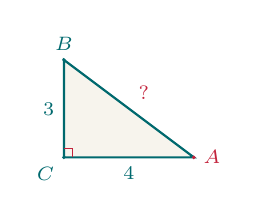
\begin{tikzpicture}[scale=0.55]
  \coordinate (C) at (0, 0);
  \coordinate (A) at (3.0, 0);
  \coordinate (B) at (0, 2.25);
  \fill[brandLightBlue] (C) -- (A) -- (B) -- cycle;
  \draw[thick, color=brandNavy] (C) -- (A) -- (B) -- cycle;
  \draw[color=brandCrimson, line width=0.5pt] ($(C)!0.2cm!(A)$) -- ($($(C)!0.2cm!(A)$)+($(C)!0.2cm!(B)$)-(C)$) -- ($(C)!0.2cm!(B)$);
  \fill[brandCrimson] (A) circle (1.3pt) node[right, font=\fontsize{7.5}{7.5}\selectfont] {$A$};
  \fill[brandNavy] (B) circle (1.3pt) node[above, font=\fontsize{7.5}{7.5}\selectfont] {$B$};
  \fill[brandNavy] (C) circle (1.3pt) node[below left, font=\fontsize{7.5}{7.5}\selectfont] {$C$};
  \node[below, font=\fontsize{7.5}{7.5}\selectfont\bfseries, color=brandNavy] at (1.5, 0) {$4$};
  \node[left, font=\fontsize{7.5}{7.5}\selectfont\bfseries, color=brandNavy] at (0, 1.1) {$3$};
  \node[above right, font=\fontsize{7.5}{7.5}\selectfont\bfseries, color=brandCrimson] at (1.5, 1.1) {$?$};
\end{tikzpicture}
\vspace{-4pt}
\end{center}

% --- Problem 02 ---
\exhead{2} ក្នុងត្រីកោណកែង $MNP$ កែងត្រង់ $P$ មាន $MN = 2\text{ cm}$ និង $\sin N = \dfrac{1}{2}$ ៖
\begin{khsubitems}
  \item[\khlabel{ក}] គណនារង្វាស់ជ្រុងឈម $MP$ នៃមុំ $N$ ។
  \item[\khlabel{ខ}] ទាញរកប្រវែងជ្រុងជាប់ $NP$ ដោយប្រើទ្រឹស្ដីបទពីតាគ័រ ។
\end{khsubitems}

\begin{center}
\vspace{-4pt}
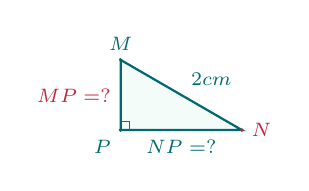
\begin{tikzpicture}[scale=0.55]
  \coordinate (P) at (0, 0);
  \coordinate (N) at (2.8, 0);
  \coordinate (M) at (0, 1.62);
  \fill[brandTealBg] (P) -- (N) -- (M) -- cycle;
  \draw[thick, color=brandNavy] (P) -- (N) -- (M) -- cycle;
  \draw[color=brandCrimson, line width=0.5pt] ($(P)!0.2cm!(N)$) -- ($($(P)!0.2cm!(N)$)+($(P)!0.2cm!(M)$)-(P)$) -- ($(P)!0.2cm!(M)$);
  \fill[brandCrimson] (N) circle (1.3pt) node[right, font=\fontsize{7.5}{7.5}\selectfont] {$N$};
  \fill[brandNavy] (M) circle (1.3pt) node[above, font=\fontsize{7.5}{7.5}\selectfont] {$M$};
  \fill[brandNavy] (P) circle (1.3pt) node[below left, font=\fontsize{7.5}{7.5}\selectfont] {$P$};
  \node[above right, font=\fontsize{7.5}{7.5}\selectfont\bfseries, color=brandNavy] at (1.4, 0.8) {$2\text{ cm}$};
  \node[left, font=\fontsize{7.5}{7.5}\selectfont\bfseries, color=brandCrimson] at (0, 0.8) {$MP=?$};
  \node[below, font=\fontsize{7.5}{7.5}\selectfont\bfseries, color=brandNavy] at (1.4, 0) {$NP=?$};
\end{tikzpicture}
\vspace{-4pt}
\end{center}

\columnbreak

% --- Problem 03 (Textbook Ex 1 p.219) ---
\exhead{3} គេមានត្រីកោណ $ABC$ កែងត្រង់ $B$ និងជ្រុង $AB = 24\text{ cm}$ ។ ដោយស្គាល់ $\tan A = \dfrac{3}{4}$ ៖
\begin{khsubitems}
  \item[\khlabel{ក}] គណនាប្រវែងជ្រុងឈម $BC$ ។
  \item[\khlabel{ខ}] គណនាប្រវែង $AC$ រួចទាញរក $\sin A$ និង $\cos A$ ។
\end{khsubitems}

\begin{center}
\vspace{-4pt}
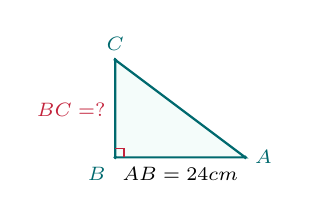
\begin{tikzpicture}[scale=0.55]
  \coordinate (B) at (0, 0);
  \coordinate (A) at (3.0, 0);
  \coordinate (C) at (0, 2.25);
  \fill[brandTealBg] (B) -- (A) -- (C) -- cycle;
  \draw[thick, color=brandNavy] (B) -- (A) -- (C) -- cycle;
  \draw[color=brandCrimson, line width=0.5pt] ($(B)!0.2cm!(A)$) -- ($($(B)!0.2cm!(A)$)+($(B)!0.2cm!(C)$)-(B)$) -- ($(B)!0.2cm!(C)$);
  \node[below, font=\fontsize{7.5}{7.5}\selectfont\bfseries] at (1.5, 0) {$AB = 24\text{ cm}$};
  \node[left, font=\fontsize{7.5}{7.5}\selectfont\bfseries, color=brandCrimson] at (0, 1.1) {$BC = ?$};
  \fill[brandNavy] (A) circle (1.3pt) node[right, font=\fontsize{7.5}{7.5}\selectfont] {$A$};
  \fill[brandNavy] (B) circle (1.3pt) node[below left, font=\fontsize{7.5}{7.5}\selectfont] {$B$};
  \fill[brandNavy] (C) circle (1.3pt) node[above, font=\fontsize{7.5}{7.5}\selectfont] {$C$};
\end{tikzpicture}
\vspace{-4pt}
\end{center}

% --- Problem 04 (Textbook Practicum 1 p.217) ---
\exhead{4} គណនាតម្លៃ $\sin\alpha$ តាមរូបត្រីកោណកែងខាងក្រោម ៖
\begin{khsubitems}
  \item[\khlabel{ក}] រូបទី ១ (ស្គាល់ជ្រុងឈម $3\text{ cm}$ និងអ៊ីប៉ូតេនុស $5\text{ cm}$)
  \item[\khlabel{ខ}] រូបទី ២ (ស្គាល់ជ្រុងឈម $4$ និងជ្រុងជាប់ $15$)
\end{khsubitems}

\begin{center}
\vspace{-4pt}
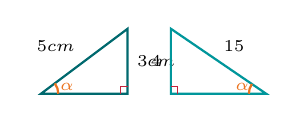
\begin{tikzpicture}[scale=0.55]
  % Triangle 1
  \coordinate (C1) at (2.0, 0);
  \coordinate (A1) at (0, 0);
  \coordinate (B1) at (2.0, 1.5);
  \draw[thick, color=brandNavy] (A1) -- (C1) -- (B1) -- cycle;
  \draw[color=brandCrimson, line width=0.4pt] ($(C1)!0.16cm!(A1)$) -- ($($(C1)!0.16cm!(A1)$)+($(C1)!0.16cm!(B1)$)-(C1)$) -- ($(C1)!0.16cm!(B1)$);
  \node[right, font=\fontsize{6.5}{6.5}\selectfont\bfseries] at (2.0, 0.75) {$3\text{ cm}$};
  \node[above left, font=\fontsize{6.5}{6.5}\selectfont\bfseries] at (1.0, 0.75) {$5\text{ cm}$};
  \draw[color=koreaOrange, thick] ($(A1)+(0.4,0)$) arc (0:36.8:0.4);
  \node[color=koreaOrange, font=\fontsize{6.5}{6.5}\selectfont\bfseries] at (0.6, 0.15) {$\alpha$};

  % Triangle 2
  \begin{scope}[xshift=3.0cm]
    \coordinate (C2) at (0, 0);
    \coordinate (A2) at (2.2, 0);
    \coordinate (B2) at (0, 1.5);
    \draw[thick, color=brandBlue] (C2) -- (A2) -- (B2) -- cycle;
    \draw[color=brandCrimson, line width=0.4pt] ($(C2)!0.16cm!(A2)$) -- ($($(C2)!0.16cm!(A2)$)+($(C2)!0.16cm!(B2)$)-(C2)$) -- ($(C2)!0.16cm!(B2)$);
    \node[left, font=\fontsize{6.5}{6.5}\selectfont\bfseries] at (0, 0.75) {$4$};
    \node[above right, font=\fontsize{6.5}{6.5}\selectfont\bfseries] at (1.0, 0.75) {$15$};
    \draw[color=koreaOrange, thick] ($(A2)+(-0.4,0)$) arc (180:145.7:0.4);
    \node[color=koreaOrange, font=\fontsize{6.5}{6.5}\selectfont\bfseries] at (1.65, 0.15) {$\alpha$};
  \end{scope}
\end{tikzpicture}
\end{center}

\end{multicols}

% =========================================================================
% ទំព័រទី ២ ៖ ផ្នែកទី ២ ផលធៀបត្រីកោណមាត្រនៃមុំពិសេស (30°, 45°, 60°)
% =========================================================================
\newpage

\khsection{២}{ផលធៀបត្រីកោណមាត្រនៃមុំពិសេស ($30^\circ, 45^\circ, 60^\circ$)}

\begin{khboxorange}
  \noindent
  \begin{minipage}[c]{0.54\textwidth}
    \centering
    {\small\kml\bfseries\color{brandNavy}តារាងតម្លៃផលធៀបត្រីកោណមាត្រនៃមុំពិសេស}\\[3pt]
    \renewcommand{\arraystretch}{1.3}
    \begin{tabular}{|c|c|c|c|}
      \hline
      \rowcolor{koreaTeal!25}
      \textbf{ផលធៀប $\backslash$ មុំ} & $\boldsymbol{30^\circ}$ & $\boldsymbol{45^\circ}$ & $\boldsymbol{60^\circ}$ \\
      \hline
      $\boldsymbol{\sin\alpha}$ & $\dfrac{1}{2}$ & $\dfrac{\sqrt{2}}{2}$ & $\dfrac{\sqrt{3}}{2}$ \\
      \hline
      $\boldsymbol{\cos\alpha}$ & $\dfrac{\sqrt{3}}{2}$ & $\dfrac{\sqrt{2}}{2}$ & $\dfrac{1}{2}$ \\
      \hline
      $\boldsymbol{\tan\alpha}$ & $\dfrac{\sqrt{3}}{3}$ & $1$ & $\sqrt{3}$ \\
      \hline
    \end{tabular}
  \end{minipage}\hfill
  \begin{minipage}[c]{0.44\textwidth}
    \begin{itemize}[leftmargin=10pt, itemsep=3pt, topsep=1pt, parsep=0pt]
      \item[\color{brandCrimson}\ding{228}] \textbf{ប្រភពតម្លៃមុំ $30^\circ$ និង $60^\circ$ ៖} បានមកពីការគូសកម្ពស់ពុះចែកត្រីកោណសម័ង្សដែលមានជ្រុង $a$ ជាពីរចំណែកកែងស្មើគ្នា ។
      \item[\color{brandNavy}\ding{228}] \textbf{ប្រភពតម្លៃមុំ $45^\circ$ ៖} បានមកពីត្រីកោណកែងសមបាតដែលមានជ្រុងកែងស្មើគ្នា $a$ និងអ៊ីប៉ូតេនុស $a\sqrt{2}$ ។
    \end{itemize}
  \end{minipage}
\end{khboxorange}

\vspace{1pt}
% Misconceptions / Memory Trick
\begin{khtipbox}
  \begin{minipage}[c]{0.66\textwidth}
    {\bfseries\color{brandCrimson}\ding{169}\ គន្លឹះចងចាំតារាងមុំពិសេសងាយៗមិនបាច់ទន្ទេញ ៖}
    \begin{itemize}[leftmargin=10pt, itemsep=2pt, topsep=1pt, parsep=0pt]
      \item[\ding{70}] \textbf{ក្បួនរាប់ឫសការ៉េសម្រាប់ស៊ីនុស ($\sin$) ៖} 
      $\sin 0^\circ = \frac{\sqrt{0}}{2} = 0$,\ \ $\sin 30^\circ = \frac{\sqrt{1}}{2} = \frac{1}{2}$,\ \ $\sin 45^\circ = \frac{\sqrt{2}}{2}$,\ \ $\sin 60^\circ = \frac{\sqrt{3}}{2}$,\ \ $\sin 90^\circ = \frac{\sqrt{4}}{2} = 1$ ។
      \item[\ding{70}] \textbf{កូស៊ីនុស ($\cos$) ៖} សរសេរច្រាសលំដាប់ពីស្តាំទៅឆ្វេងនៃតម្លៃស៊ីនុសវិញ ($1, \frac{\sqrt{3}}{2}, \frac{\sqrt{2}}{2}, \frac{1}{2}, 0$) ។
      \item[\ding{70}] \textbf{តង់សង់ ($\tan$) ៖} យកតម្លៃ $\sin$ ចែកនឹង $\cos$ រៀងៗខ្លួន តាមរូបមន្ត $\tan\alpha = \frac{\sin\alpha}{\cos\alpha}$ ។
    \end{itemize}
  \end{minipage}\hfill
  \begin{minipage}[c]{0.32\textwidth}
    \centering
    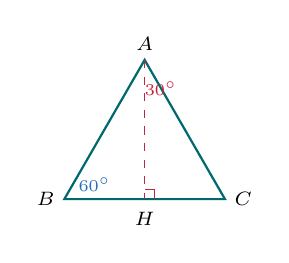
\begin{tikzpicture}[scale=0.85]
      % Triangle 30-60-90
      \coordinate (H) at (0, 0);
      \coordinate (B) at (-1.2, 0);
      \coordinate (C) at (1.2, 0);
      \coordinate (A) at (0, 2.08);
      \draw[thick, color=brandNavy] (B) -- (C) -- (A) -- cycle;
      \draw[dashed, color=brandCrimson] (A) -- (H);
      \draw[color=brandCrimson, line width=0.4pt] ($(H)!0.15cm!(C)$) -- ($($(H)!0.15cm!(C)$)+($(H)!0.15cm!(A)$)-(H)$) -- ($(H)!0.15cm!(A)$);
      \node[below, font=\fontsize{7}{7}\selectfont] at (0, -0.05) {$H$};
      \node[left, font=\fontsize{7}{7}\selectfont] at (B) {$B$};
      \node[right, font=\fontsize{7}{7}\selectfont] at (C) {$C$};
      \node[above, font=\fontsize{7}{7}\selectfont] at (A) {$A$};
      \node[font=\fontsize{6.5}{6.5}\selectfont, color=brandCrimson] at (0.24, 1.65) {$30^\circ$};
      \node[font=\fontsize{6.5}{6.5}\selectfont, color=koreaBlue] at (-0.75, 0.22) {$60^\circ$};
    \end{tikzpicture}
  \end{minipage}
\end{khtipbox}

\vspace{2pt}
% Practice Problems 05-08 for Section 2 (Multicols 2)
\begin{multicols}{2}

% --- Problem 05 ---
\exhead{5} គណនាតម្លៃនៃកន្សោមគណិតវិទ្យាខាងក្រោមដោយប្រើតម្លៃមុំពិសេស ៖
\begin{khsubitems}
  \item[\khlabel{ក}] $A = 2\sin 30^\circ + 4\cos 60^\circ - \tan 45^\circ$
  \item[\khlabel{ខ}] $B = \sin^2 45^\circ + \cos^2 45^\circ$
  \item[\khlabel{គ}] $C = \dfrac{\sin 60^\circ}{\cos 30^\circ} + \sqrt{3}\tan 30^\circ$
\end{khsubitems}

\begin{center}
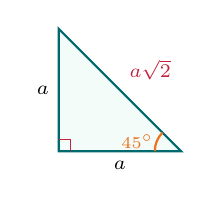
\begin{tikzpicture}[scale=0.74]
  \coordinate (C) at (0, 0);
  \coordinate (B) at (2.1, 0);
  \coordinate (A) at (0, 2.1);
  \fill[brandTealBg] (C) -- (B) -- (A) -- cycle;
  \draw[thick, color=brandNavy] (C) -- (B) -- (A) -- cycle;
  \draw[color=brandCrimson, line width=0.5pt] ($(C)!0.2cm!(B)$) -- ($($(C)!0.2cm!(B)$)+($(C)!0.2cm!(A)$)-(C)$) -- ($(C)!0.2cm!(A)$);
  \node[below, font=\fontsize{7.5}{7.5}\selectfont] at (1.05, 0) {$a$};
  \node[left, font=\fontsize{7.5}{7.5}\selectfont] at (0, 1.05) {$a$};
  \node[above right, font=\fontsize{7.5}{7.5}\selectfont\color{brandCrimson}] at (1.05, 1.05) {$a\sqrt{2}$};
  \draw[color=koreaOrange, thick] ($(B)+(-0.45,0)$) arc (180:135:0.45);
  \node[color=koreaOrange, font=\fontsize{6.5}{6.5}\selectfont\bfseries] at (1.35, 0.16) {$45^\circ$};
\end{tikzpicture}
\end{center}

% --- Problem 06 (Textbook Ex 2 p.219) ---
\exhead{6} តាមរូបខាងក្រោម ចូរគណនារង្វាស់ជ្រុង $x$ និង $y$ ៖
\begin{khsubitems}
  \item[\khlabel{ក}] ក្នុងរូបទី ១ រកប្រវែង $x$ និង $QR$ ។
  \item[\khlabel{ខ}] ក្នុងរូបទី ២ រកប្រវែង $y$ និង $ST$ ។
\end{khsubitems}

\begin{center}
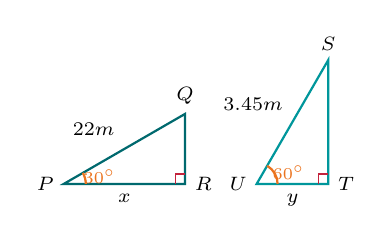
\begin{tikzpicture}[scale=0.70]
  % Figure 1
  \coordinate (R) at (2.2, 0);
  \coordinate (P) at (0, 0);
  \coordinate (Q) at (2.2, 1.27);
  \draw[thick, color=brandNavy] (P) -- (R) -- (Q) -- cycle;
  \draw[color=brandCrimson, line width=0.4pt] ($(R)!0.18cm!(P)$) -- ($($(R)!0.18cm!(P)$)+($(R)!0.18cm!(Q)$)-(R)$) -- ($(R)!0.18cm!(Q)$);
  \node[below, font=\fontsize{7}{7}\selectfont\bfseries] at (1.1, 0) {$x$};
  \node[above left, font=\fontsize{7}{7}\selectfont\bfseries] at (1.1, 0.7) {$22\text{ m}$};
  \draw[color=koreaOrange, thick] ($(P)+(0.4,0)$) arc (0:30:0.4);
  \node[color=koreaOrange, font=\fontsize{6.5}{6.5}\selectfont\bfseries] at (0.65, 0.14) {$30^\circ$};
  \node[left, font=\fontsize{7}{7}\selectfont] at (P) {$P$};
  \node[right, font=\fontsize{7}{7}\selectfont] at (R) {$R$};
  \node[above, font=\fontsize{7}{7}\selectfont] at (Q) {$Q$};

  % Figure 2
  \begin{scope}[xshift=3.5cm]
    \coordinate (T) at (1.3, 0);
    \coordinate (U) at (0, 0);
    \coordinate (S) at (1.3, 2.25);
    \draw[thick, color=brandBlue] (U) -- (T) -- (S) -- cycle;
    \draw[color=brandCrimson, line width=0.4pt] ($(T)!0.18cm!(U)$) -- ($($(T)!0.18cm!(U)$)+($(T)!0.18cm!(S)$)-(T)$) -- ($(T)!0.18cm!(S)$);
    \node[below, font=\fontsize{7}{7}\selectfont\bfseries] at (0.65, 0) {$y$};
    \node[above left, font=\fontsize{7}{7}\selectfont\bfseries] at (0.65, 1.15) {$3.45\text{ m}$};
    \draw[color=koreaOrange, thick] ($(U)+(0.38,0)$) arc (0:60:0.38);
    \node[color=koreaOrange, font=\fontsize{6.5}{6.5}\selectfont\bfseries] at (0.58, 0.2) {$60^\circ$};
    \node[left, font=\fontsize{7}{7}\selectfont] at (U) {$U$};
    \node[right, font=\fontsize{7}{7}\selectfont] at (T) {$T$};
    \node[above, font=\fontsize{7}{7}\selectfont] at (S) {$S$};
  \end{scope}
\end{tikzpicture}
\end{center}

\columnbreak

% --- Problem 07 (Textbook Ex 3 & Ex 15 p.219-220) ---
\exhead{7} តាមរូបខាងស្តាំ គេមាន $\triangle ABC$ កែងត្រង់ $A$ ដែល $BC = 4\text{ m}$ និង $\angle C = 30^\circ$ ៖
\begin{khsubitems}
  \item[\khlabel{ក}] គណនាប្រវែងជ្រុង $AC$ និង $AB$ ។
  \item[\khlabel{ខ}] រកផ្ទៃក្រឡានៃត្រីកោណ $ABC$ នោះ ។
\end{khsubitems}

\begin{center}
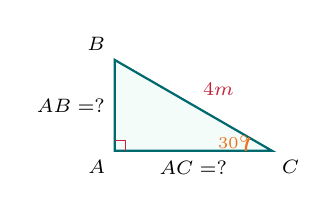
\begin{tikzpicture}[scale=0.74]
  \coordinate (A) at (0, 0);
  \coordinate (C) at (2.7, 0);
  \coordinate (B) at (0, 1.56);
  \fill[brandTealBg] (A) -- (C) -- (B) -- cycle;
  \draw[thick, color=brandNavy] (A) -- (C) -- (B) -- cycle;
  \draw[color=brandCrimson, line width=0.4pt] ($(A)!0.18cm!(C)$) -- ($($(A)!0.18cm!(C)$)+($(A)!0.18cm!(B)$)-(A)$) -- ($(A)!0.18cm!(B)$);
  \node[above right, font=\fontsize{7.5}{7.5}\selectfont\bfseries, color=brandCrimson] at (1.35, 0.78) {$4\text{ m}$};
  \node[below, font=\fontsize{7.5}{7.5}\selectfont\bfseries] at (1.35, 0) {$AC=?$};
  \node[left, font=\fontsize{7.5}{7.5}\selectfont\bfseries] at (0, 0.78) {$AB=?$};
  \draw[color=koreaOrange, thick] ($(C)+(-0.45,0)$) arc (180:150:0.45);
  \node[color=koreaOrange, font=\fontsize{6.5}{6.5}\selectfont\bfseries] at (2.05, 0.15) {$30^\circ$};
  \node[below left, font=\fontsize{7.5}{7.5}\selectfont] at (A) {$A$};
  \node[below right, font=\fontsize{7.5}{7.5}\selectfont] at (C) {$C$};
  \node[above left, font=\fontsize{7.5}{7.5}\selectfont] at (B) {$B$};
\end{tikzpicture}
\end{center}

% --- Problem 08 (Textbook Practicum 2 p.218) ---
\exhead{8} ក្នុងត្រីកោណកែង $QRS$ ដែលកែងត្រង់ $Q$ មានជ្រុង $QR = 3\text{ cm}$ និង $\angle R = 30^\circ$ ៖
\begin{khsubitems}
  \item[\khlabel{ក}] គណនារង្វាស់អ៊ីប៉ូតេនុស $RS$ ។
  \item[\khlabel{ខ}] គណនាប្រវែងជ្រុង $QS$ ។
\end{khsubitems}

\begin{center}
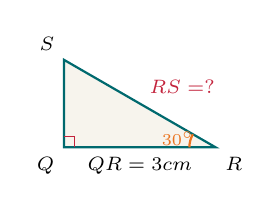
\begin{tikzpicture}[scale=0.74]
  \coordinate (Q) at (0, 0);
  \coordinate (R) at (2.6, 0);
  \coordinate (S) at (0, 1.5);
  \fill[brandLightBlue] (Q) -- (R) -- (S) -- cycle;
  \draw[thick, color=brandNavy] (Q) -- (R) -- (S) -- cycle;
  \draw[color=brandCrimson, line width=0.4pt] ($(Q)!0.18cm!(R)$) -- ($($(Q)!0.18cm!(R)$)+($(Q)!0.18cm!(S)$)-(Q)$) -- ($(Q)!0.18cm!(S)$);
  \node[below, font=\fontsize{7.5}{7.5}\selectfont\bfseries] at (1.3, 0) {$QR = 3\text{ cm}$};
  \node[above right, font=\fontsize{7.5}{7.5}\selectfont\bfseries, color=brandCrimson] at (1.3, 0.75) {$RS = ?$};
  \draw[color=koreaOrange, thick] ($(R)+(-0.45,0)$) arc (180:150:0.45);
  \node[color=koreaOrange, font=\fontsize{6.5}{6.5}\selectfont\bfseries] at (1.95, 0.15) {$30^\circ$};
  \node[below left, font=\fontsize{7.5}{7.5}\selectfont] at (Q) {$Q$};
  \node[below right, font=\fontsize{7.5}{7.5}\selectfont] at (R) {$R$};
  \node[above left, font=\fontsize{7.5}{7.5}\selectfont] at (S) {$S$};
\end{tikzpicture}
\end{center}

\end{multicols}

% =========================================================================
% ទំព័រទី ៣ ៖ ផ្នែកទី ៣ អនុវត្តន៍ជាក់ស្ដែងលើទីវាល (មុំងើប មុំទម្លាក់)
% =========================================================================
\newpage

\khsection{៣}{អនុវត្តន៍ជាក់ស្ដែង ៖ មុំងើប មុំទម្លាក់ និងការគណនាកម្ពស់}

\begin{khboxorange}
  \begin{minipage}[c]{0.62\textwidth}
    ក្នុងការវាស់វែងជាក់ស្ដែងលើទីវាល គេប្រើផលធៀបត្រីកោណមាត្រដើម្បីគណនាកម្ពស់ ឬចម្ងាយដែលមិនអាចវាស់ដោយផ្ទាល់បាន ៖
    \begin{itemize}[leftmargin=12pt, itemsep=3pt, topsep=2pt, parsep=0pt]
      \item[\color{brandCrimson}\ding{228}] \textbf{មុំងើប (Angle of Elevation) ៖} ជាមុំដែលបង្កើតឡើងរវាង \textbf{ខ្សែដេកផ្ដេក} នៃភ្នែកអ្នកសង្កេត និងខ្សែបន្ទាត់សម្លឹង \textbf{ទៅលើ} ឆ្ពោះទៅកាន់វត្ថុ ។
      \item[\color{brandNavy}\ding{228}] \textbf{មុំទម្លាក់ (Angle of Depression) ៖} ជាមុំដែលបង្កើតឡើងរវាង \textbf{ខ្សែដេកផ្ដេក} នៃភ្នែកអ្នកសង្កេត និងខ្សែបន្ទាត់សម្លឹង \textbf{ចុះក្រោម} ឆ្ពោះទៅកាន់វត្ថុ ។
    \end{itemize}
  \end{minipage}\hfill
  \begin{minipage}[c]{0.36\textwidth}
    \centering
    \begin{tikzpicture}[scale=0.90]
      % Observer eye O
      \coordinate (O) at (0, 1.15);
      \coordinate (H1) at (3.4, 1.15);
      \coordinate (T) at (3.1, 2.35);
      \coordinate (B) at (3.1, 0.0);
      % Horizontal line
      \draw[dashed, thick, color=gray!80] (O) -- (H1) node[right, font=\fontsize{7}{7}\selectfont] {ខ្សែដេក};
      % Sight line up
      \draw[thick, color=brandCrimson] (O) -- (T) node[above right, font=\fontsize{7}{7}\selectfont\bfseries] {កំពូលវត្ថុ};
      % Sight line down
      \draw[thick, color=brandNavy] (O) -- (B) node[below right, font=\fontsize{7}{7}\selectfont\bfseries] {បាតវត្ថុ};
      % Angles
      \draw[thick, color=brandCrimson] ($(O)+(0.65,0)$) arc (0:21.5:0.65);
      \node[color=brandCrimson, font=\fontsize{6.5}{6.5}\selectfont\kml\bfseries] at (1.05, 1.4) {មុំងើប};
      \draw[thick, color=brandNavy] ($(O)+(0.65,0)$) arc (0:-20:0.65);
      \node[color=brandNavy, font=\fontsize{6.5}{6.5}\selectfont\kml\bfseries] at (1.05, 0.9) {មុំទម្លាក់};
      \fill[black] (O) circle (1.5pt) node[left, font=\fontsize{7}{7}\selectfont\kml] {ភ្នែក};
    \end{tikzpicture}
  \end{minipage}
\end{khboxorange}

\vspace{1pt}
% Misconception Box for Section 3
\begin{khtipbox}
  {\bfseries\color{brandCrimson}\ding{169}\ ចំណាំពិសេសក្នុងការគណនាមុំងើប និងមុំទម្លាក់ ៖}
  \begin{itemize}[leftmargin=10pt, itemsep=2pt, topsep=1pt, parsep=0pt]
    \item[\ding{70}] មុំងើប និងមុំទម្លាក់ ត្រូវតែគិតធៀបនឹង \textcolor{brandCrimson}{\textbf{ខ្សែដេកផ្ដេក (Horizontal Line)}} ជានិច្ច មិនមែនធៀបនឹងខ្សែឈរ ឬជញ្ជាំងឡើយ ។
    \item[\ding{70}] មុំងើបពីចំណុច $A$ ទៅចំណុច $B$ គឺស្មើនឹងមុំទម្លាក់ពីចំណុច $B$ មកចំណុច $A$ ជានិច្ច ពីព្រោះវាជាមុំឆ្លាស់ក្នុងរវាងខ្សែដេកស្របគ្នាទាំងពីរ ។
  \end{itemize}
\end{khtipbox}

\vspace{2pt}
% Practice Problems 09-12 for Section 3 (Multicols 2)
\begin{multicols}{2}

% --- Problem 09 (Tree Problem p.218) ---
\exhead{9} គេវាស់កម្ពស់ដើមឈើមួយដើម ដោយដឹងថាស្រមោលរបស់វាធៀបនឹងដីរាបបានមុំ $60^\circ$ ហើយចម្ងាយពីគល់ដើមឈើទៅចុងស្រមោលលើដីស្មើ $10.5\text{ m}$ ៖
\begin{khsubitems}
  \item[\khlabel{ក}] កំណត់រូបមន្តផលធៀបត្រីកោណមាត្រដែលត្រូវប្រើ ។
  \item[\khlabel{ខ}] គណនាកម្ពស់ដើមឈើ (យក $\sqrt{3} \approx 1.732$) ។
\end{khsubitems}

\begin{center}
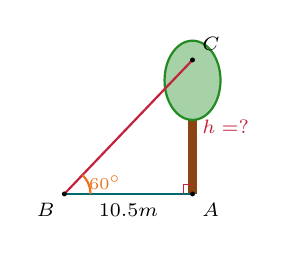
\begin{tikzpicture}[scale=0.74]
  \coordinate (A) at (2.2, 0);
  \coordinate (B) at (0, 0);
  \coordinate (C) at (2.2, 2.3);
  \draw[line width=3pt, color=treeBrown] (A) -- (C);
  \draw[fill=treeGreen!40, draw=treeGreen, thick] (2.2, 1.95) ellipse (0.48cm and 0.68cm);
  \draw[thick, color=brandNavy] (B) -- (A);
  \draw[thick, color=brandCrimson] (B) -- (C);
  \draw[color=brandCrimson, line width=0.4pt] ($(A)!0.16cm!(B)$) -- ($($(A)!0.16cm!(B)$)+($(A)!0.16cm!(C)$)-(A)$) -- ($(A)!0.16cm!(C)$);
  \draw[color=koreaOrange, thick] ($(B)+(0.45,0)$) arc (0:46:0.45);
  \node[color=koreaOrange, font=\fontsize{6.5}{6.5}\selectfont\bfseries] at (0.7, 0.2) {$60^\circ$};
  \node[below, font=\fontsize{7}{7}\selectfont\bfseries] at (1.1, 0) {$10.5\text{ m}$};
  \node[right, font=\fontsize{7}{7}\selectfont\bfseries, color=brandCrimson] at (2.2, 1.15) {$h=?$};
  \fill[black] (A) circle (1.2pt) node[below right, font=\fontsize{7}{7}\selectfont] {$A$};
  \fill[black] (B) circle (1.2pt) node[below left, font=\fontsize{7}{7}\selectfont] {$B$};
  \fill[black] (C) circle (1.2pt) node[above right, font=\fontsize{7}{7}\selectfont] {$C$};
\end{tikzpicture}
\end{center}

% --- Problem 10 (Textbook Ex 4 p.219) ---
\exhead{10} ជណ្ដើរផ្ទះមួយមានប្រវែង $5\text{ m}$ ត្រូវបានគេដាក់ផ្អែកលើជញ្ជាំងផ្ទះ ដោយឱ្យជើងជណ្ដើរឃ្លាតពីជញ្ជាំងចម្ងាយ $3\text{ m}$ ៖
\begin{khsubitems}
  \item[\khlabel{ក}] គណនាកូស៊ីនុសនៃមុំ $\alpha$ ដែលជណ្ដើរផ្ដុំជាមួយដី ។
  \item[\khlabel{ខ}] គណនាកម្ពស់ជញ្ជាំងដែលចុងជណ្ដើរដាក់ដល់ ។
\end{khsubitems}

\begin{center}
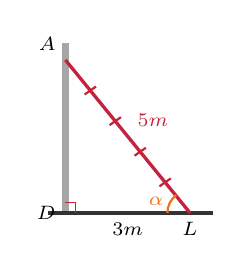
\begin{tikzpicture}[scale=0.72]
  \coordinate (D) at (0, 0);
  \coordinate (L) at (2.2, 0);
  \coordinate (A) at (0, 2.7);
  \draw[line width=2.5pt, color=gray!70] (D) -- (0, 3.0);
  \draw[line width=1.4pt, color=black!80] (-0.3, 0) -- (2.6, 0);
  \draw[very thick, color=brandCrimson] (L) -- (A);
  \foreach \i in {0.2, 0.4, 0.6, 0.8} {
    \draw[thick, color=brandCrimson] ($($(L)!\i!(A)$)+(-0.1, -0.07)$) -- ($($(L)!\i!(A)$)+(0.1, 0.07)$);
  }
  \draw[color=brandCrimson, line width=0.4pt] ($(D)!0.18cm!(L)$) -- ($($(D)!0.18cm!(L)$)+($(D)!0.18cm!(A)$)-(D)$) -- ($(D)!0.18cm!(A)$);
  \node[below, font=\fontsize{7.5}{7.5}\selectfont\bfseries] at (1.1, 0) {$3\text{ m}$};
  \node[above right, font=\fontsize{7.5}{7.5}\selectfont\bfseries, color=brandCrimson] at (1.1, 1.35) {$5\text{ m}$};
  \node[left, font=\fontsize{7.5}{7.5}\selectfont] at (D) {$D$};
  \node[below, font=\fontsize{7.5}{7.5}\selectfont] at (L) {$L$};
  \node[above left, font=\fontsize{7.5}{7.5}\selectfont] at (A) {$A$};
  \draw[color=koreaOrange, thick] ($(L)+(-0.4,0)$) arc (180:128:0.4);
  \node[color=koreaOrange, font=\fontsize{7}{7}\selectfont\bfseries] at (1.6, 0.2) {$\alpha$};
\end{tikzpicture}
\end{center}

\columnbreak

% --- Problem 11 (Textbook Ex 5 p.219) ---
\exhead{11} ត្រីកោណសមបាតមួយមានរង្វាស់បាតស្មើ $12\text{ cm}$ និងកម្ពស់គូសចេញពីកំពូលមានរង្វាស់ $14.1\text{ cm}$ ៖
\begin{khsubitems}
  \item[\khlabel{ក}] គណនាតង់សង់នៃមុំបាតនីមួយៗ ។
  \item[\khlabel{ខ}] រកប្រវែងជ្រុងទ្រេតនៃត្រីកោណសមបាតនោះ ។
\end{khsubitems}

\begin{center}
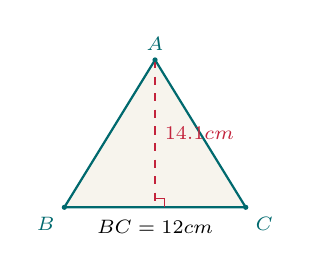
\begin{tikzpicture}[scale=0.72]
  \coordinate (B) at (-1.6, 0);
  \coordinate (C) at (1.6, 0);
  \coordinate (A) at (0, 2.6);
  \coordinate (H) at (0, 0);
  \fill[brandLightBlue] (B) -- (C) -- (A) -- cycle;
  \draw[thick, color=brandNavy] (B) -- (C) -- (A) -- cycle;
  \draw[dashed, thick, color=brandCrimson] (A) -- (H);
  \draw[color=brandCrimson, line width=0.4pt] ($(H)!0.16cm!(C)$) -- ($($(H)!0.16cm!(C)$)+($(H)!0.16cm!(A)$)-(H)$) -- ($(H)!0.16cm!(A)$);
  \node[below, font=\fontsize{7.5}{7.5}\selectfont\bfseries] at (0, -0.05) {$BC = 12\text{ cm}$};
  \node[right, font=\fontsize{7.5}{7.5}\selectfont\bfseries, color=brandCrimson] at (0, 1.3) {$14.1\text{ cm}$};
  \fill[brandNavy] (A) circle (1.3pt) node[above, font=\fontsize{7.5}{7.5}\selectfont] {$A$};
  \fill[brandNavy] (B) circle (1.3pt) node[below left, font=\fontsize{7.5}{7.5}\selectfont] {$B$};
  \fill[brandNavy] (C) circle (1.3pt) node[below right, font=\fontsize{7.5}{7.5}\selectfont] {$C$};
\end{tikzpicture}
\end{center}

% --- Problem 12 (Textbook Ex 13 p.220) ---
\exhead{12} បង្គោលខ្សែភ្លើងមួយដើមមានកម្ពស់ $6\text{ m}$ ។ គេចងខ្សែដែកស្ទោងមួយខ្សែមានប្រវែង $15\text{ m}$ ពីចុងបង្គោលមកដី (ដូចរូប) ៖
\begin{khsubitems}
  \item[\khlabel{ក}] គណនាស៊ីនុសនៃមុំរវាងខ្សែស្ទោង និងដីរាប ។
  \item[\khlabel{ខ}] គណនាចម្ងាយពីគល់បង្គោលទៅចំណុចចងខ្សែលើដី ។
\end{khsubitems}

\begin{center}
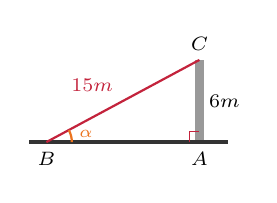
\begin{tikzpicture}[scale=0.72]
  \coordinate (A) at (2.7, 0);
  \coordinate (B) at (0, 0);
  \coordinate (C) at (2.7, 1.45);
  \draw[line width=3pt, color=gray!80] (A) -- (C);
  \draw[line width=1.2pt, color=black!80] (-0.3, 0) -- (3.2, 0);
  \draw[thick, color=brandCrimson] (B) -- (C);
  \draw[color=brandCrimson, line width=0.4pt] ($(A)!0.18cm!(B)$) -- ($($(A)!0.18cm!(B)$)+($(A)!0.18cm!(C)$)-(A)$) -- ($(A)!0.18cm!(C)$);
  \node[right, font=\fontsize{7.5}{7.5}\selectfont\bfseries] at (2.7, 0.72) {$6\text{ m}$};
  \node[above left, font=\fontsize{7.5}{7.5}\selectfont\bfseries, color=brandCrimson] at (1.35, 0.72) {$15\text{ m}$};
  \node[below, font=\fontsize{7.5}{7.5}\selectfont] at (B) {$B$};
  \node[below, font=\fontsize{7.5}{7.5}\selectfont] at (A) {$A$};
  \node[above, font=\fontsize{7.5}{7.5}\selectfont] at (C) {$C$};
  \draw[color=koreaOrange, thick] ($(B)+(0.45,0)$) arc (0:28:0.45);
  \node[color=koreaOrange, font=\fontsize{6.5}{6.5}\selectfont\bfseries] at (0.7, 0.15) {$\alpha$};
\end{tikzpicture}
\end{center}

\end{multicols}

% =========================================================================
% ទំព័រទី ៤ ៖ ផ្នែកទី ៣ (បន្ត) លំហាត់អនុវត្តជាក់ស្ដែងលើទីវាល
% =========================================================================
\newpage

\khsection{៤}{កម្រងលំហាត់អនុវត្តជាក់ស្ដែងលើទីវាលបន្ថែម (បន្ត)}

\begin{multicols}{2}

% --- Problem 13 (Textbook Ex 14 p.220) ---
\exhead{13} ដំបូលផ្ទះមួយរាងត្រីកោណសមបាតដែលមានប្រវែងទ្រនុងដំបូល $RS = RT = 8\text{ m}$ និងកម្ពស់ដំបូលពីកំពូលមកបាតស្មើ $6\text{ m}$ ៖
\begin{khsubitems}
  \item[\khlabel{ក}] គណនាស៊ីនុសនៃមុំលំអៀង $\angle RST$ នៃដំបូល ។
  \item[\khlabel{ខ}] គណនាប្រវែងបាតដំបូល $ST$ ទាំងមូល ។
\end{khsubitems}

\begin{center}
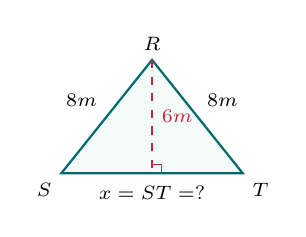
\begin{tikzpicture}[scale=0.72]
  \coordinate (S) at (-1.6, 0);
  \coordinate (T) at (1.6, 0);
  \coordinate (R) at (0, 2.0);
  \coordinate (M) at (0, 0);
  \fill[brandTealBg] (S) -- (T) -- (R) -- cycle;
  \draw[thick, color=brandNavy] (S) -- (T) -- (R) -- cycle;
  \draw[dashed, thick, color=brandCrimson] (R) -- (M);
  \draw[color=brandCrimson, line width=0.4pt] ($(M)!0.16cm!(T)$) -- ($($(M)!0.16cm!(T)$)+($(M)!0.16cm!(R)$)-(M)$) -- ($(M)!0.16cm!(R)$);
  \node[above left, font=\fontsize{7.5}{7.5}\selectfont\bfseries] at (-0.8, 1.0) {$8\text{ m}$};
  \node[above right, font=\fontsize{7.5}{7.5}\selectfont\bfseries] at (0.8, 1.0) {$8\text{ m}$};
  \node[right, font=\fontsize{7.5}{7.5}\selectfont\bfseries, color=brandCrimson] at (0, 1.0) {$6\text{ m}$};
  \node[below, font=\fontsize{7.5}{7.5}\selectfont\bfseries] at (0, -0.05) {$x = ST = ?$};
  \node[above, font=\fontsize{7.5}{7.5}\selectfont] at (R) {$R$};
  \node[below left, font=\fontsize{7.5}{7.5}\selectfont] at (S) {$S$};
  \node[below right, font=\fontsize{7.5}{7.5}\selectfont] at (T) {$T$};
\end{tikzpicture}
\end{center}

% --- Problem 14 (Textbook Ex 7 p.219) ---
\exhead{14} ក្មេងម្នាក់បង្ហោះខ្លែងដោយលែងខ្សែប្រវែង $7\text{ m}$ ហើយខ្សែនោះផ្ដុំជាមួយខ្សែដេកបានមុំ $20^\circ$ (ដឹងថា $\sin 20^\circ \approx 0.342$) ៖
\begin{khsubitems}
  \item[\khlabel{ក}] គណនាកម្ពស់ខ្លែងធៀបនឹងដីរាប ។
  \item[\khlabel{ខ}] បើចង់ឱ្យខ្លែងឡើងបានកម្ពស់ $4\text{ m}$ ដោយមុំដដែល តើត្រូវលែងខ្សែប្រវែងប៉ុន្មាន?
\end{khsubitems}

\begin{center}
\begin{tikzpicture}[scale=0.70]
  \coordinate (O) at (0, 0);
  \coordinate (H) at (2.7, 0);
  \coordinate (K) at (2.7, 0.98);
  \draw[line width=1.2pt, color=black!80] (-0.3, 0) -- (3.2, 0);
  \draw[thick, color=brandCrimson] (O) -- (K);
  \draw[dashed, thick, color=brandNavy] (K) -- (H);
  \draw[color=brandCrimson, line width=0.4pt] ($(H)!0.16cm!(O)$) -- ($($(H)!0.16cm!(O)$)+($(H)!0.16cm!(K)$)-(H)$) -- ($(H)!0.16cm!(K)$);
  \node[above left, font=\fontsize{7.5}{7.5}\selectfont\bfseries, color=brandCrimson] at (1.35, 0.52) {$7\text{ m}$};
  \node[right, font=\fontsize{7.5}{7.5}\selectfont\bfseries, color=brandNavy] at (2.7, 0.48) {$h=?$};
  \draw[color=koreaOrange, thick] ($(O)+(0.45,0)$) arc (0:20:0.45);
  \node[color=koreaOrange, font=\fontsize{6.5}{6.5}\selectfont\bfseries] at (0.75, 0.13) {$20^\circ$};
  \fill[brandCrimson] (K) circle (1.8pt) node[above right=1pt, font=\fontsize{7}{7}\selectfont\kml] {ខ្លែង};
\end{tikzpicture}
\end{center}

% --- Problem 15 (Textbook Ex 8 p.219) ---
\exhead{15} រថយន្តមួយបើកបរលើផ្លូវទេរឡើងចំណោតភ្នំបានចម្ងាយ $1.5\text{ km}$ ដោយផ្លូវនោះផ្ដុំជាមួយប្លង់ដេកបានមុំ $5^\circ$ (ដឹងថា $\sin 5^\circ \approx 0.0872$) ៖
\begin{khsubitems}
  \item[\khlabel{ក}] គណនាកម្ពស់ដែលរថយន្តនោះឡើងបាន (គិតជា $\text{m}$) ។
  \item[\khlabel{ខ}] គណនាចម្ងាយផ្លូវដេកដែលរថយន្តបានធ្វើដំណើរ (យក $\cos 5^\circ \approx 0.996$) ។
\end{khsubitems}

\begin{center}
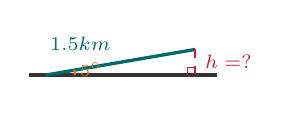
\begin{tikzpicture}[scale=0.68]
  \coordinate (A) at (0, 0);
  \coordinate (B) at (2.8, 0);
  \coordinate (C) at (2.8, 0.48);
  \draw[line width=1.2pt, color=black!80] (-0.3, 0) -- (3.2, 0);
  \draw[very thick, color=brandNavy] (A) -- (C);
  \draw[dashed, thick, color=brandCrimson] (C) -- (B);
  \draw[color=brandCrimson, line width=0.4pt] ($(B)!0.15cm!(A)$) -- ($($(B)!0.15cm!(A)$)+($(B)!0.15cm!(C)$)-(B)$) -- ($(B)!0.15cm!(C)$);
  \node[above left, font=\fontsize{7.5}{7.5}\selectfont\bfseries, color=brandNavy] at (1.4, 0.28) {$1.5\text{ km}$};
  \node[right, font=\fontsize{7.5}{7.5}\selectfont\bfseries, color=brandCrimson] at (2.8, 0.24) {$h=?$};
  \draw[color=koreaOrange, thick] ($(A)+(0.55,0)$) arc (0:10:0.55);
  \node[color=koreaOrange, font=\fontsize{6.5}{6.5}\selectfont\bfseries] at (0.85, 0.11) {$5^\circ$};
\end{tikzpicture}
\end{center}

\columnbreak

% --- Problem 16 (Textbook Ex 9 p.220) ---
\exhead{16} ជើងខ្សែចងស្រាក់ដងក្ដោងទូកមួយ ផ្ដុំជាមួយផ្ទៃរាបស្មើនៃទូកបានមុំ $50^\circ$ ។ រកប្រវែងដងក្ដោង ដោយដឹងថាគម្លាតពីគល់ដងក្ដោងទៅជើងខ្សែមានចម្ងាយ $3\text{ m}$ (យក $\tan 50^\circ \approx 1.192$) ។

\begin{center}
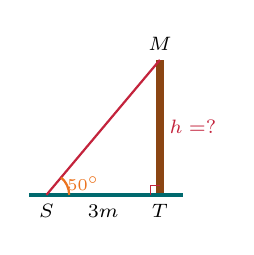
\begin{tikzpicture}[scale=0.72]
  \coordinate (T) at (2.0, 0);
  \coordinate (S) at (0, 0);
  \coordinate (M) at (2.0, 2.38);
  \draw[line width=2.8pt, color=treeBrown] (T) -- (M);
  \draw[line width=1.3pt, color=brandNavy] (-0.3, 0) -- (2.4, 0);
  \draw[thick, color=brandCrimson] (S) -- (M);
  \draw[color=brandCrimson, line width=0.4pt] ($(T)!0.16cm!(S)$) -- ($($(T)!0.16cm!(S)$)+($(T)!0.16cm!(M)$)-(T)$) -- ($(T)!0.16cm!(M)$);
  \node[below, font=\fontsize{7.5}{7.5}\selectfont\bfseries] at (1.0, 0) {$3\text{ m}$};
  \node[right, font=\fontsize{7.5}{7.5}\selectfont\bfseries, color=brandCrimson] at (2.0, 1.2) {$h=?$};
  \draw[color=koreaOrange, thick] ($(S)+(0.4,0)$) arc (0:50:0.4);
  \node[color=koreaOrange, font=\fontsize{6.5}{6.5}\selectfont\bfseries] at (0.65, 0.2) {$50^\circ$};
  \node[below, font=\fontsize{7.5}{7.5}\selectfont] at (S) {$S$};
  \node[below, font=\fontsize{7.5}{7.5}\selectfont] at (T) {$T$};
  \node[above, font=\fontsize{7.5}{7.5}\selectfont] at (M) {$M$};
\end{tikzpicture}
\end{center}

% --- Problem 17 (Textbook Ex 12 p.220) ---
\exhead{17} តើជណ្ដើរ $AP$ ត្រូវមានរង្វាស់ប៉ុន្មាន ដើម្បីដាក់ផ្អែកនឹងជញ្ជាំង $AB$ មួយដែលមានកម្ពស់ $2.5\text{ m}$ ដោយមុំរវាងជណ្ដើរ និងដីរាបស្មើនឹង $40^\circ$ (ដឹងថា $\sin 40^\circ \approx 0.643$) ?

\begin{center}
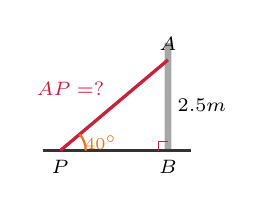
\begin{tikzpicture}[scale=0.72]
  \coordinate (B) at (1.9, 0);
  \coordinate (P) at (0, 0);
  \coordinate (A) at (1.9, 1.6);
  \draw[line width=2.5pt, color=gray!70] (B) -- (1.9, 1.9);
  \draw[line width=1.2pt, color=black!80] (-0.3, 0) -- (2.3, 0);
  \draw[very thick, color=brandCrimson] (P) -- (A);
  \draw[color=brandCrimson, line width=0.4pt] ($(B)!0.16cm!(P)$) -- ($($(B)!0.16cm!(P)$)+($(B)!0.16cm!(A)$)-(B)$) -- ($(B)!0.16cm!(A)$);
  \node[right, font=\fontsize{7.5}{7.5}\selectfont\bfseries] at (1.9, 0.8) {$2.5\text{ m}$};
  \node[above left, font=\fontsize{7.5}{7.5}\selectfont\bfseries, color=brandCrimson] at (0.95, 0.8) {$AP=?$};
  \draw[color=koreaOrange, thick] ($(P)+(0.45,0)$) arc (0:40:0.45);
  \node[color=koreaOrange, font=\fontsize{6.5}{6.5}\selectfont\bfseries] at (0.72, 0.15) {$40^\circ$};
  \node[below, font=\fontsize{7.5}{7.5}\selectfont] at (P) {$P$};
  \node[below, font=\fontsize{7.5}{7.5}\selectfont] at (B) {$B$};
  \node[above, font=\fontsize{7.5}{7.5}\selectfont] at (A) {$A$};
\end{tikzpicture}
\end{center}

% --- Problem 18 (Textbook Ex 17 p.220) ---
\exhead{18} ពហុកោណ $ABCDE$ មាន $\angle EAC = \angle ACD = 90^\circ$ ហើយ $AE = 6\text{ cm}$ ។ ចំណុច $B$ ស្ថិតនៅលើអង្កត់ $AC$ ដែល $AB = 8\text{ cm}$, $EB = 10\text{ cm}$, $BD = 5\text{ cm}$ និង $\angle EBD = 90^\circ$ ៖
\begin{khsubitems}
  \item[\khlabel{ក}] គណនាផ្ទៃក្រឡាចតុកោណពុះ $ABDE$ ។
  \item[\khlabel{ខ}] គណនាប្រវែងអង្កត់ $ED$ និង $DC$ ។
\end{khsubitems}

\begin{center}
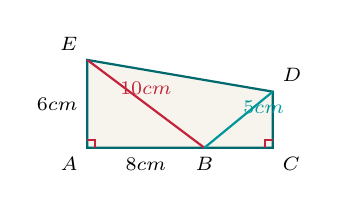
\begin{tikzpicture}[scale=0.62]
  \coordinate (A) at (0, 0);
  \coordinate (E) at (0, 1.8);
  \coordinate (B) at (2.4, 0);
  \coordinate (C) at (3.8, 0);
  \coordinate (D) at (3.8, 1.15);

  \fill[brandLightBlue] (A) -- (C) -- (D) -- (E) -- cycle;
  \draw[thick, color=brandNavy] (A) -- (C) -- (D) -- (E) -- cycle;
  \draw[thick, color=brandCrimson] (E) -- (B);
  \draw[thick, color=brandBlue] (B) -- (D);

  % Right angles
  \draw[color=brandCrimson, line width=0.4pt] ($(A)!0.16cm!(C)$) -- ($($(A)!0.16cm!(C)$)+($(A)!0.16cm!(E)$)-(A)$) -- ($(A)!0.16cm!(E)$);
  \draw[color=brandCrimson, line width=0.4pt] ($(C)!0.16cm!(A)$) -- ($($(C)!0.16cm!(A)$)+($(C)!0.16cm!(D)$)-(C)$) -- ($(C)!0.16cm!(D)$);

  \node[left, font=\fontsize{7}{7}\selectfont\bfseries] at (0, 0.9) {$6\text{ cm}$};
  \node[below, font=\fontsize{7}{7}\selectfont\bfseries] at (1.2, 0) {$8\text{ cm}$};
  \node[above, font=\fontsize{7}{7}\selectfont\bfseries, color=brandCrimson] at (1.2, 0.9) {$10\text{ cm}$};
  \node[above right, font=\fontsize{7}{7}\selectfont\bfseries, color=brandBlue] at (3.0, 0.5) {$5\text{ cm}$};

  \node[below left, font=\fontsize{7}{7}\selectfont] at (A) {$A$};
  \node[above left, font=\fontsize{7}{7}\selectfont] at (E) {$E$};
  \node[below, font=\fontsize{7.5}{7.5}\selectfont] at (B) {$B$};
  \node[below right, font=\fontsize{7.5}{7.5}\selectfont] at (C) {$C$};
  \node[above right, font=\fontsize{7.5}{7.5}\selectfont] at (D) {$D$};
\end{tikzpicture}
\end{center}

\end{multicols}

\end{document}
